%%%%%%%%%%%%%%%%%%%%%%%%%%%%% Thesis.tex %%%%%%%%%%%%%%%%%%%%%%%%%%%%%%%
%                                                                      %
%  ---------- Master of Science Dissertation template ----------       %
%                                                                      %
%  Template for the Master Thesis according to the regulations         %
%  published by the Academic Board (Direcção Académica) at IST.        %
%                                                                      %
%  For up-to-date guide, please refer to the official website          %
%
% https://tecnico.ulisboa.pt/pt/ensino/estudar-no-tecnico/informacoes-academicas/dissertacao-de-mestrado/
%                                                                      %
%       Andre C. Marta                                                 %
%       Area Cientifica de Mecanica Aplicada e Aeroespacial            %
%       Departamento de Engenharia Mecanica                            %
%       Instituto Superior Tecnico                                     %
%       Av. Rovisco Pais                                               %
%       1049-001 Lisboa                                                %
%       Portugal                                                       %
%       Tel: +351 21 841 9469                                          %
%                        3469 (extension)                              %
%       Email: andre.marta@tecnico.ulisboa.pt                          %
%                                                                      %
%  Created:       Jan 20, 2011                                         %
%  Last Modified: JUn 29, 2022                                         %
%                                                                      %
%%%%%%%%%%%%%%%%%%%%%%%%%%%%%%%%%%%%%%%%%%%%%%%%%%%%%%%%%%%%%%%%%%%%%%%%
%  Revision history                                                    %
%  v1 - 2011/01/24 - original template                                 %
%  v2 - 2012/10/30 - new IST image and glossary support                %
%  v3 - 2013/12/10 - update according to 2012/13 official guide        %
%  v4 - 2014/02/28 - new default for bibliography style                %
%  v5 - 2014/05/07 - update according to 2013/14 official guide        %
%  v6 - 2015/07/02 - cover page format fixed,                          %
%                    contents page numbering fixed,                    %
%                    better language support,                          %
%                    enhanced examples of tables,                      %
%                    new option for appendix page numbering format,    %
%                    custom bibliography style                         %
%  v7 - 2018/02/19 - multiple citations compressed                     %
%  v8 - 2019/05/13 - added examples (pseudo-code)                      %
%  v9 - 2020/03/03 - added French language support                     %
%                    indented first paragraphs                         %
%  v10- 2021/01/29 - place caption above table                         %
%  v11- 2022/06/29 - included Declaration of original work             %
%%%%%%%%%%%%%%%%%%%%%%%%%%%%%%%%%%%%%%%%%%%%%%%%%%%%%%%%%%%%%%%%%%%%%%%%
%                                                                      %
% To generate the PDF file, type "make" at the terminal prompt.        %
%                                                                      %
% The IST template LaTeX package was created by the author             %
% and it can be downloaded from:                                       %
% https://fenix.ist.utl.pt/homepage/ist31052/                          %
%                                                                      %
% The external packages can be downloaded from                         %
% the Comprehensive TeX Archive Network at http://www.ctan.org/        %
%                                                                      %
% List of LaTex symbols:                                               %
% http://www.ctan.org/tex-archive/info/symbols/comprehensive/          %
%                                                                      %
% Help with LaTex can be found at                                      %
% http://www.giss.nasa.gov/tools/latex/ltx-2.html                      %
% http://en.wikibooks.org/wiki/LaTeX                                   %
%%%%%%%%%%%%%%%%%%%%%%%%%%%%%%%%%%%%%%%%%%%%%%%%%%%%%%%%%%%%%%%%%%%%%%%%

%%%%%%%%%%%%%%%%%%%%%%%%%%%%%%%%%%%%%%%%%%%%%%%%%%%%%%%%%%%%%%%%%%%%%%%%
%     Preamble                                                         %
%%%%%%%%%%%%%%%%%%%%%%%%%%%%%%%%%%%%%%%%%%%%%%%%%%%%%%%%%%%%%%%%%%%%%%%%

% ----------------------------------------------------------------------
%  Set the document class
% ----------------------------------------------------------------------
\documentclass[10pt,a4paper,twoside]{report}

% ----------------------------------------------------------------------
% Define external packages, language, margins, fonts and new commands
% ----------------------------------------------------------------------
%%%%%%%%%%%%%%%%%%%%%%%%%%%%%%%%%%%%%%%%%%%%%%%%%%%%%%%%%%%%%%%%%%%%%%%%
%                                                                      %
%     File: Thesis_Preamble.tex                                        %
%     Tex Master: Thesis.tex                                           %
%                                                                      %
%     Author: Andre C. Marta                                           %
%     Last modified : 29 Jun 2022                                      %
%                                                                      %
%%%%%%%%%%%%%%%%%%%%%%%%%%%%%%%%%%%%%%%%%%%%%%%%%%%%%%%%%%%%%%%%%%%%%%%%

% 'natbib' package
%
% Flexible bibliography support.
% http://www.ctan.org/tex-archive/macros/latex/contrib/natbib/
%
% > produce author-year style citations
%
% \citet  and \citep  for textual and parenthetical citations, respectively
% \citet* and \citep* that print the full author list, and not just the abbreviated one
% \citealt is the same as \citet but without parentheses. Similarly, \citealp is \citep without parentheses
% \citeauthor
% \citeyear
% \citeyearpar
%
%% natbib options can be provided when package is loaded \usepackage[options]{natbib}
%%
%% Following options are valid:
%%
%%   round  -  round parentheses are used (default)
%%   square -  square brackets are used   [option]
%%   curly  -  curly braces are used      {option}
%%   angle  -  angle brackets are used    <option>
%%   semicolon  -  multiple citations separated by semi-colon (default)
%%   colon  - same as semicolon, an earlier confusion
%%   comma  -  separated by comma
%%   authoryear - for author–year citations (default)
%%   numbers-  selects numerical citations
%%   super  -  numerical citations as superscripts, as in Nature
%%   sort   -  sorts multiple citations according to order in ref. list
%%   sort&compress   -  like sort, but also compresses numerical citations
%%   compress - compresses without sorting
%%
% ******************************* SELECT *******************************
%\usepackage{natbib}          % <<<<< References in alphabetical list Correia, Silva, ...
\usepackage[numbers,sort&compress]{natbib} % <<<<< References in numbered list [1],[2],...
% ******************************* SELECT *******************************


% 'notoccite' package
%
% Prevent trouble from citations in table of contents, etc.
% http://ctan.org/pkg/notoccite
%
% > If you have \cite com­mands in \sec­tion-like com­mands, or in \cap­tion,
%   the ci­ta­tion will also ap­pear in the ta­ble of con­tents, or list of what­ever.
%   If you are also us­ing an un­srt-like bib­li­og­ra­phy style, these ci­ta­tions will
%   come at the very start of the bib­li­og­ra­phy, which is con­fus­ing. This pack­age
%   sup­presses the ef­fect.
%
\usepackage{notoccite}


% ----------------------------------------------------------------------
% Define document language.
% ----------------------------------------------------------------------

% 'inputenc' package
%
% Accept different input encodings.
% http://www.ctan.org/tex-archive/macros/latex/base/
%
% > allows typing non-english text in LaTeX sources.
%
% ******************************* SELECT *******************************
%\usepackage[latin1]{inputenc} % <<<<< Windows
\usepackage[utf8]{inputenc}   % <<<<< Linux
% ******************************* SELECT *******************************


% 'babel' package
%
% Multilingual support for Plain TeX or LaTeX.
% http://www.ctan.org/tex-archive/macros/latex/required/babel/
%
% > sets the variable names according to the language selected
%
% ******************************* SELECT *******************************
%\usepackage[portuguese]{babel} % <<<<< Portuguese
\usepackage[english]{babel} % <<<<< English
%\usepackage[francais]{babel} % <<<<< French (requires package texlive-lang-french)
% ******************************* SELECT *******************************


% List of LaTeX variable names: \abstractname, \appendixname, \bibname,
%   \chaptername, \contentsname, \listfigurename, \listtablename, ...)
% http://www.tex.ac.uk/cgi-bin/texfaq2html?label=fixnam
%
% Changing the words babel uses (uncomment and redefine as necessary...)
%
\newcommand{\acknowledgments}{@undefined} % new LaTeX variable name
%
% > English
%
\addto\captionsenglish{\renewcommand{\acknowledgments}{Acknowledgments}}
%\addto\captionsenglish{\renewcommand{\contentsname}{Contents}}
%\addto\captionsenglish{\renewcommand{\listtablename}{List of Tables}}
%\addto\captionsenglish{\renewcommand{\listfigurename}{List of Figures}}
%\addto\captionsenglish{\renewcommand{\nomname}{Nomenclature}}
%\addto\captionsenglish{\renewcommand{\glossaryname}{Glossary}}
%\addto\captionsenglish{\renewcommand{\acronymname}{List of Acronyms}}
%\addto\captionsenglish{\renewcommand{\bibname}{References}} % Bibliography
%\addto\captionsenglish{\renewcommand{\appendixname}{Appendix}}

% > French
%
\addto\captionsfrench{\renewcommand{\acknowledgments}{Remerciements}}
%\addto\captionsfrench{\renewcommand{\contentsname}{Table des matières}}
%\addto\captionsfrench{\renewcommand{\listtablename}{Liste des tableaux}}
\addto\captionsfrench{\renewcommand{\listfigurename}{Liste des figures}} % Table des figures
%\addto\captionsfrench{\renewcommand{\nomname}{Nomenclature}}
%\addto\captionsfrench{\renewcommand{\glossaryname}{Glossaire}}
%\addto\captionsfrench{\renewcommand{\acronymname}{Liste des acronymes}}
%\addto\captionsfrench{\renewcommand{\bibname}{Bibliographie}}
%\addto\captionsfrench{\renewcommand{\appendixname}{Annexe}}

% > Portuguese
%
\addto\captionsportuguese{\renewcommand{\acknowledgments}{Agradecimentos}}
%\addto\captionsportuguese{\renewcommand{\contentsname}{Conte\'{u}do}}
%\addto\captionsportuguese{\renewcommand{\listtablename}{Lista de Figuras}}
%\addto\captionsportuguese{\renewcommand{\listfigurename}{Lista de Tabelas}}
\addto\captionsportuguese{\renewcommand{\nomname}{Lista de S\'{i}mbolos}} % Nomenclatura
%\addto\captionsportuguese{\renewcommand{\glossary}{Gloss\'{a}rio}}
%\addto\captionsportuguese{\renewcommand{\acronymname}{Lista de Abrevia\c{c}\~{o}es}}
%\addto\captionsportuguese{\renewcommand{\bibname}{Refer\^{e}ncias}} % Bibliografia
%\addto\captionsportuguese{\renewcommand{\appendixname}{Anexo}} % Apendice


% ----------------------------------------------------------------------
% Define cover fields in both english and portuguese.
% ----------------------------------------------------------------------
%
\newcommand{\coverThesis}{@undefined} % new LaTeX variable name
\newcommand{\coverSupervisors}{@undefined} % new LaTeX variable name
\newcommand{\coverExaminationCommittee}{@undefined} % new LaTeX variable name
\newcommand{\coverChairperson}{@undefined} % new LaTeX variable name
\newcommand{\coverSupervisor}{@undefined} % new LaTeX variable name
\newcommand{\coverMemberCommittee}{@undefined} % new LaTeX variable name
% > English
\addto\captionsenglish{\renewcommand{\coverThesis}{Thesis to obtain the Master of Science Degree in}}
\addto\captionsenglish{\renewcommand{\coverSupervisors}{Supervisor(s)}}
\addto\captionsenglish{\renewcommand{\coverExaminationCommittee}{Examination Committee}}
\addto\captionsenglish{\renewcommand{\coverChairperson}{Chairperson}}
\addto\captionsenglish{\renewcommand{\coverSupervisor}{Supervisor}}
\addto\captionsenglish{\renewcommand{\coverMemberCommittee}{Member of the Committee}}
% > French
\addto\captionsfrench{\renewcommand{\coverThesis}{Th\`ese pour l'obtention du Maîtrise des Sciences en}}
\addto\captionsfrench{\renewcommand{\coverSupervisors}{Directeur(s) de th\`ese}}
\addto\captionsfrench{\renewcommand{\coverExaminationCommittee}{Jury}}
\addto\captionsfrench{\renewcommand{\coverChairperson}{Pr\'esident}}
\addto\captionsfrench{\renewcommand{\coverSupervisor}{Directeur de th\`ese}}
\addto\captionsfrench{\renewcommand{\coverMemberCommittee}{Rapporteur}}
% > Portuguese
\addto\captionsportuguese{\renewcommand{\coverThesis}{Disserta\c{c}\~{a}o para obten\c{c}\~{a}o do Grau de Mestre em}}
\addto\captionsportuguese{\renewcommand{\coverSupervisors}{Orientador(es)}}
\addto\captionsportuguese{\renewcommand{\coverExaminationCommittee}{J\'{u}ri}}
\addto\captionsportuguese{\renewcommand{\coverChairperson}{Presidente}}
\addto\captionsportuguese{\renewcommand{\coverSupervisor}{Orientador}}
\addto\captionsportuguese{\renewcommand{\coverMemberCommittee}{Vogal}}


% ----------------------------------------------------------------------
% Define Declaration of original work in both english and portuguese.
% ----------------------------------------------------------------------
%
\newcommand{\declarationTitle}{@undefined} % new LaTeX variable name
\newcommand{\declarationText}{@undefined}  % new LaTeX variable name
% > English
\addto\captionsenglish{\renewcommand{\declarationTitle}{Declaration}}
\addto\captionsenglish{\renewcommand{\declarationText}{I declare that this document is an original work of my own authorship and that it fulfills all the requirements of the Code of Conduct and Good Practices of the Universidade de Lisboa.}}
% > Portuguese
\addto\captionsportuguese{\renewcommand{\declarationTitle}{Declara\c{c}\~{a}o}}
\addto\captionsportuguese{\renewcommand{\declarationText}{Declaro que o presente documento \'{e} um trabalho original da minha autoria e que cumpre todos os requisitos do C\'{o}digo de Conduta e Boas Pr\'{a}ticas da Universidade de Lisboa.}}


% ----------------------------------------------------------------------
% Define default and cover page fonts.
% ----------------------------------------------------------------------

% Use Arial font as default
%
\renewcommand{\rmdefault}{phv}
\renewcommand{\sfdefault}{phv}

% Define cover page fonts
%
%         encoding     family       series      shape
%  \usefont{T1}     {phv}=helvetica  {b}=bold    {n}=normal
%                   {ptm}=times      {m}=normal  {sl}=slanted
%                                                {it}=italic
% see more examples at
% https://www.overleaf.com/learn/latex/Font_typefaces
% https://tug.org/FontCatalogue/
%
\def\FontLn{% 16 pt normal
  \usefont{T1}{phv}{m}{n}\fontsize{16pt}{16pt}\selectfont}
\def\FontLb{% 16 pt bold
  \usefont{T1}{phv}{b}{n}\fontsize{16pt}{16pt}\selectfont}
\def\FontMn{% 14 pt normal
  \usefont{T1}{phv}{m}{n}\fontsize{14pt}{14pt}\selectfont}
\def\FontMb{% 14 pt bold
  \usefont{T1}{phv}{b}{n}\fontsize{14pt}{14pt}\selectfont}
\def\FontSn{% 12 pt normal
  \usefont{T1}{phv}{m}{n}\fontsize{12pt}{12pt}\selectfont}


% ----------------------------------------------------------------------
% Define page margins and line spacing.
% ----------------------------------------------------------------------

% 'geometry' package
%
% Flexible and complete interface to document dimensions.
% http://www.ctan.org/tex-archive/macros/latex/contrib/geometry/
%
% > set the page margins (2.5cm minimum in every side, as per IST rules)
%
\usepackage{geometry}	
\geometry{verbose,tmargin=2.5cm,bmargin=2.5cm,lmargin=2.5cm,rmargin=2.5cm}

% 'setspace' package
%
% Set space between lines.
% http://www.ctan.org/tex-archive/macros/latex/contrib/setspace/
%
% > allow setting line spacing (line spacing of 1.5, as per IST rules)
%
\usepackage{setspace}
\renewcommand{\baselinestretch}{1.5}


% ----------------------------------------------------------------------
% Define paragraph formating.
% ----------------------------------------------------------------------

% 'indentfirst' package
%
% Indent first paragraph after section header.
% https://ctan.org/pkg/indentfirst
%
% > indent all paragraphs (as per IST rules)
%
\usepackage{indentfirst}	


% ----------------------------------------------------------------------
% Include external packages.
% Note that not all of these packages may be available on all system
% installations. If necessary, include the .sty files locally in
% the <jobname>.tex file directory.
% ----------------------------------------------------------------------

% 'graphicx' package
%
% Enhanced support for graphics.
% http://www.ctan.org/tex-archive/macros/latex/required/graphics/
%
% > extends arguments of the \includegraphics command
%
\usepackage{graphicx}


% 'color' package
%
% Colour control for LaTeX documents.
% http://www.ctan.org/tex-archive/macros/latex/required/graphics/
%
% > defines color macros: \color{<color name>}
%
%\usepackage{color}


% 'amsmath' package
%
% Mathematical enhancements for LaTeX.
% http://www.ctan.org/tex-archive/macros/latex/required/amslatex/
%
% > American Mathematical Society plain Tex macros
%
\usepackage{amsmath}  % AMS mathematical facilities for LaTeX.
\usepackage{amsthm}   % Typesetting theorems (AMS style).
\usepackage{amsfonts} % 
\usepackage{mathrsfs}
\usepackage{amsmath,fourier}
\usepackage{amssymb}
\theoremstyle{remark}
\newtheorem{remark}{Remark}
\theoremstyle{plain}
\newtheorem{proposition}{Proposition}

% 'wrapfig' package
%
% Produces figures which text can flow around.
% http://www.ctan.org/tex-archive/macros/latex/contrib/wrapfig/
%
% > wrap figures/tables in text (i.e., Di Vinci style)
%
% \usepackage{wrapfig}


% 'subfigure' package
%
% Deprecated: Figures divided into subfigures.
% http://www.ctan.org/tex-archive/obsolete/macros/latex/contrib/subfigure/
%
% > subcaptions for subfigures
%
\usepackage{subfigure}


% 'subfigmat' package
%
% Automates layout when using the subfigure package.
% http://www.ctan.org/tex-archive/macros/latex/contrib/subfigmat/
%
% > matrices of similar subfigures
%
\usepackage{subfigmat}


% 'url' package
%
% Verbatim with URL-sensitive line breaks.
% http://www.ctan.org/tex-archive/macros/latex/contrib/url/
%
% > URLs in BibTex
%
% \usepackage{url}


% 'varioref' package
%
% Intelligent page references.
% http://www.ctan.org/tex-archive/macros/latex/required/tools/
%
% > smart page, figure, table and equation referencing
%
%\usepackage{varioref}


% 'dcolumn' package
%
% Align on the decimal point of numbers in tabular columns.
% http://www.ctan.org/tex-archive/macros/latex/required/tools/
%
% > decimal-aligned tabular math columns
%
\usepackage{dcolumn}
\newcolumntype{d}{D{.}{.}{-1}} % column aligned by the point separator '.'
\newcolumntype{e}{D{E}{E}{-1}} % column aligned by the exponent 'E'


% 'verbatim' package
%
% Reimplementation of and extensions to LaTeX verbatim.
% http://www.ctan.org/tex-archive/macros/latex/required/tools/
%
% > provides the verbatim environment (\begin{verbatim},\end{verbatim})
%   and a comment environment (\begin{comment},  \end{comment})
%
% \usepackage{verbatim}


% 'moreverb' package
%
% Extended verbatim.
% http://www.ctan.org/tex-archive/macros/latex/contrib/moreverb/
%
% > supports tab expansion and line numbering
%
% \usepackage{moreverb}



% 'nomencl' package
%
% Produce lists of symbols as in nomenclature.
% http://www.ctan.org/tex-archive/macros/latex/contrib/nomencl/
%
% The nomencl package makes use of the MakeIndex program
% in order to produce the nomenclature list.
%
% Nomenclature
% 1) On running the file through LATEX, the command \makenomenclature
%    in the preamble instructs it to create/open the nomenclature file
%    <jobname>.nlo corresponding to the LATEX file <jobname>.tex and
%    writes the information from the \nomenclature commands to this file.
% 2) The next step is to invoke MakeIndex in order to produce the
%    <jobname>.nls file. This can be achieved by making use of the
%    command: makeindex <jobname>.nlo -s nomencl.ist -o <jobname>.nls
% 3) The last step is to invoke LATEX on the <jobname>.tex file once
%    more. There, the \printnomenclature in the document will input the
%    <jobname>.nls file and process it according to the given options.
%
% http://www-h.eng.cam.ac.uk/help/tpl/textprocessing/nomencl.pdf
%
% Nomenclature (produces *.nlo *.nls files)
\usepackage{nomencl}
\makenomenclature
%
% Group variables according to their symbol type
%
\RequirePackage{ifthen} 
\ifthenelse{\equal{\languagename}{english}}%
    { % English
    \renewcommand{\nomgroup}[1]{%
      \ifthenelse{\equal{#1}{R}}{%
        \item[\textbf{Roman symbols}]}{%
        \ifthenelse{\equal{#1}{G}}{%
          \item[\textbf{Greek symbols}]}{%
          \ifthenelse{\equal{#1}{S}}{%
            \item[\textbf{Subscripts}]}{%
            \ifthenelse{\equal{#1}{T}}{%
              \item[\textbf{Superscripts}]}{}}}}}%
    }{%
    \ifthenelse{\equal{\languagename}{french}}%
    { % French
    \renewcommand{\nomgroup}[1]{%
      \ifthenelse{\equal{#1}{R}}{%
        \item[\textbf{Symbole romains}]}{%
        \ifthenelse{\equal{#1}{G}}{%
          \item[\textbf{Symboles grecs}]}{%
          \ifthenelse{\equal{#1}{S}}{%
            \item[\textbf{Indices}]}{% lettre inférieure
            \ifthenelse{\equal{#1}{T}}{%
              \item[\textbf{Exposants}]}{}}}}}% lettre supérieure
    }{ % Portuguese
    \renewcommand{\nomgroup}[1]{%
      \ifthenelse{\equal{#1}{R}}{%
        \item[\textbf{Simbolos romanos}]}{%
        \ifthenelse{\equal{#1}{G}}{%
          \item[\textbf{Simbolos gregos}]}{%
          \ifthenelse{\equal{#1}{S}}{%
            \item[\textbf{Subscritos}]}{%
            \ifthenelse{\equal{#1}{T}}{%
              \item[\textbf{Sobrescritos}]}{}}}}}%
    }}%


% 'glossary' package
%
% Create a glossary.
% http://www.ctan.org/tex-archive/macros/latex/contrib/glossary/
%
% Glossary (produces *.glo *.ist files)
\usepackage[number=none]{glossary}
% (remove blank line between groups)
\setglossary{gloskip={}}
% (redefine glossary style file)
%\renewcommand{\istfilename}{myGlossaryStyle.ist}
\makeglossary


% 'rotating' package
%
% Rotation tools, including rotated full-page floats.
% http://www.ctan.org/tex-archive/macros/latex/contrib/rotating/
%
% > show wide figures and tables in landscape format:
%   use \begin{sidewaystable} and \begin{sidewaysfigure}
%   instead of 'table' and 'figure', respectively.
%
\usepackage{rotating}


% 'hyperref' package
%
% Extensive support for hypertext in LaTeX.
% http://www.ctan.org/tex-archive/macros/latex/contrib/hyperref/
%
% > Extends the functionality of all the LATEX cross-referencing
%   commands (including the table of contents, bibliographies etc) to
%   produce \special commands which a driver can turn into hypertext
%   links; Also provides new commands to allow the user to write adhoc
%   hypertext links, including those to external documents and URLs.
%
\usepackage[pdftex]{hyperref} % enhance documents that are to be
                              % output as HTML and PDF
\hypersetup{colorlinks,       % color text of links and anchors,
                              % eliminates borders around links
%            linkcolor=red,    % color for normal internal links
            linkcolor=black,  % color for normal internal links
            anchorcolor=black,% color for anchor text
%            citecolor=green,  % color for bibliographical citations
            citecolor=black,  % color for bibliographical citations
%            filecolor=magenta,% color for URLs which open local files
            filecolor=black,  % color for URLs which open local files
%            menucolor=red,    % color for Acrobat menu items
            menucolor=black,  % color for Acrobat menu items
%            pagecolor=red,    % color for links to other pages
            pagecolor=black,  % color for links to other pages
%            urlcolor=cyan,    % color for linked URLs
            urlcolor=black,   % color for linked URLs
	          bookmarks=true,         % create PDF bookmarks
	          bookmarksopen=false,    % don't expand bookmarks
	          bookmarksnumbered=true, % number bookmarks
	          pdftitle={Thesis},
            pdfauthor={Andre C. Marta},
            pdfsubject={Thesis Title},
            pdfkeywords={Thesis Keywords},
            pdfstartview=FitV,
            pdfdisplaydoctitle=true}


% 'hypcap' package
%
% Adjusting the anchors of captions.
% http://www.ctan.org/tex-archive/macros/latex/contrib/oberdiek/
%
% > fixes the problem with hyperref, that links to floats points
%   below the caption and not at the beginning of the float.
%
\usepackage[figure,table]{hypcap}


% 'multirow' package
%
% Create tabular cells spanning multiple rows
% http://www.ctan.org/pkg/multirow
%
\usepackage{multirow}


% 'booktabs' package
%
% Publication quality tables in LaTeX
% http://www.ctan.org/pkg/booktabs
%
% > en­hance the qual­ity of ta­bles in LaTeX, pro­vid­ing ex­tra com­mands.
%
% \renewcommand{\arraystretch}{<ratio>} % space between rows
%
\usepackage{booktabs}
%\newcommand{\ra}[1]{\renewcommand{\arraystretch}{#1}}


% 'pdfpages' package
%
% Include PDF documents in LaTeX
% http://www.ctan.org/pkg/pdfpages
%
% > in­clu­sion of ex­ter­nal multi-page PDF doc­u­ments in LaTeX doc­u­ments.
%   Pages may be freely se­lected and sim­i­lar to psnup it is pos­si­ble to put
%   sev­eral log­i­cal pages onto each sheet of pa­per.
%
% \includepdf{filename.pdf}
% \includepdf[pages={4-9},nup=2x3,landscape=true]{filename.pdf}
%
\usepackage{pdfpages}


% 'algorithmicx' package
%
% The algorithmic style you always wanted
% https://ctan.org/pkg/algorithmicx
%
% > provides many possibilities to customizethe layout of algorithms.  You can use one of the predefined layouts(pseudocode,pascalandcand others), with or without modifications,or you can define a completely new layout for your specific needs
%
\usepackage{algorithm}
\usepackage{algpseudocode}


% ----------------------------------------------------------------------
% Define new commands to assure consistent treatment throughout document
% ----------------------------------------------------------------------

\newcommand{\ud}{\mathrm{d}}                % total derivative
\newcommand{\degree}{\ensuremath{^\circ\,}} % degrees

% Abbreviations

\newcommand{\mcol}{\multicolumn}            % table format

\newcommand{\eqnref}[1]{(\ref{#1})}
\newcommand{\class}[1]{\texttt{#1}}
\newcommand{\package}[1]{\texttt{#1}}
\newcommand{\file}[1]{\texttt{#1}}
\newcommand{\BibTeX}{\textsc{Bib}\TeX}

% Typefaces ( example: {\bf Bold text here} )
%
% > pre-defined
%   \bf % bold face
%   \it % italic
%   \tt % typewriter
%
% > newly defined
\newcommand{\tr}[1]{{\ensuremath{\textrm{#1}}}}   % text roman
\newcommand{\tb}[1]{{\ensuremath{\textbf{#1}}}}   % text bold face
\newcommand{\ti}[1]{{\ensuremath{\textit{#1}}}}   % text italic
\newcommand{\mc}[1]{{\ensuremath{\mathcal{#1}}}}  % math calygraphy
\newcommand{\mco}[1]{{\ensuremath{\mathcalold{#1}}}}% math old calygraphy
\newcommand{\mr}[1]{{\ensuremath{\mathrm{#1}}}}   % math roman
\newcommand{\mb}[1]{{\ensuremath{\mathbf{#1}}}}   % math bold face
\newcommand{\bs}[1]{\ensuremath{\boldsymbol{#1}}} % math symbol
\def\bm#1{\mathchoice                             % math bold
  {\mbox{\boldmath$\displaystyle#1$}}%
  {\mbox{\boldmath$#1$}}%
  {\mbox{\boldmath$\scriptstyle#1$}}%
  {\mbox{\boldmath$\scriptscriptstyle#1$}}}
\newcommand{\boldcal}[1]{{\ensuremath{\boldsymbol{\mathcal{#1}}}}}% math bold calygraphy

 

%%%%%%%%%%%%%%%%%%%%%%%%%%%%%%%%%%%%%%%%%%%%%%%%%%%%%%%%%%%%%%%%%%%%%%%%
%     Begin Document                                                   %
%%%%%%%%%%%%%%%%%%%%%%%%%%%%%%%%%%%%%%%%%%%%%%%%%%%%%%%%%%%%%%%%%%%%%%%%
\begin{document}

% Set plain page style (no headers, footer with centered page number)
\pagestyle{plain}

% Set roman numbering (i,ii,...) before the start of chapters
\pagenumbering{roman}

% ----------------------------------------------------------------------
%  Cover page
% ----------------------------------------------------------------------
%%%%%%%%%%%%%%%%%%%%%%%%%%%%%%%%%%%%%%%%%%%%%%%%%%%%%%%%%%%%%%%%%%%%%%%%
%                                                                      %
%     File: Thesis_FrontCover.tex                                      %
%     Tex Master: Thesis.tex                                           %
%                                                                      %
%     Author: Andre C. Marta                                           %
%     Last modified :  2 Jul 2015                                      %
%                                                                      %
%%%%%%%%%%%%%%%%%%%%%%%%%%%%%%%%%%%%%%%%%%%%%%%%%%%%%%%%%%%%%%%%%%%%%%%%

\thispagestyle {empty}

% IST Logo - Signature A
% parameters: bb=llx lly urx ury (bounding box), width=h_length, height=v_length, angle=angle, scale=factor, clip=true/false, draft=true/false. 

\includegraphics[bb=9.5cm 11cm 0cm 0cm,scale=0.29]{Figures/Logos/IST_A_CMYK_POS}

\begin{center}

\vspace{6 cm}

{\FontLb The cylinder at spatial infinity and asymptotic charges} \\ % <<<<< EDIT TITLE
%\vspace{0.2cm}
%{\FontMn Subtitle (optional)} \\
%\vspace{1.9cm}
\vspace{2.6cm}
{\FontMb Rafael de Almeida Carvalho Pastor Pinto} \\ % <<<<< EDIT NAME
\vspace{2.0cm}
{\FontSn \coverThesis} \\
\vspace{0.3cm}
{\FontLb Engineering Physics} \\ % <<<<< EDIT COURSE
\vspace{1.0cm}
{\FontSn %
\begin{tabular}{ll}
 \coverSupervisors: & Prof. Dr. Edgar Gasperín \\ % <<<<< EDIT NAME
                    & Prof. Dr. Alex Vañó Viñuales   % <<<<< EDIT NAME
\end{tabular} } \\
\vspace{1.0cm}
{\FontMb \coverExaminationCommittee} \\
\vspace{0.3cm}
{\FontSn %
\begin{tabular}{c}
\coverChairperson:     Prof. José Pizarro de Sande e Lemos          \\ % <<<<< EDIT NAME
\coverSupervisor:      Prof. Dr. Edgar Gasperín \\ % <<<<< EDIT NAME
\coverMemberCommittee: Prof. Full Name 3           % <<<<< EDIT NAME
\end{tabular} } \\
\vspace{1.5cm}
{\FontMb Month 2023} \\ % <<<<< EDIT DATE (corresponds to date of oral examination)
%
\end{center}

 
\cleardoublepage

% ----------------------------------------------------------------------
% Dedication page (optional)
% ----------------------------------------------------------------------
%%%%%%%%%%%%%%%%%%%%%%%%%%%%%%%%%%%%%%%%%%%%%%%%%%%%%%%%%%%%%%%%%%%%%%%%
%                                                                      %
%     File: Thesis_Dedication.tex                                      %
%     Tex Master: Thesis.tex                                           %
%                                                                      %
%     Author: Andre C. Marta                                           %
%     Last modified :  2 Jul 2015                                      %
%                                                                      %
%%%%%%%%%%%%%%%%%%%%%%%%%%%%%%%%%%%%%%%%%%%%%%%%%%%%%%%%%%%%%%%%%%%%%%%%

\null\vskip5cm%
\begin{flushright}
     Quando te vi, amei-te já muito antes.\\
     Tornei a achar-te quando te encontrei.\\
     Nasci pra ti antes de haver o mundo.\\
     Não há cousa feliz ou hora alegre\\
     Que eu tenha tido pela vida fora,\\
     Que o não fosse porque te previa,\\
     Porque dormias nela tu futuro.\\
     (Fernando Pessoa) \\
     À minha namorada, Daniela, por todo o apoio e carinho que me deu durante a realização desta tese.
\end{flushright}
\vfill\newpage

 
\cleardoublepage

% ----------------------------------------------------------------------
% Declaration page (mandatory)
% ----------------------------------------------------------------------
%%%%%%%%%%%%%%%%%%%%%%%%%%%%%%%%%%%%%%%%%%%%%%%%%%%%%%%%%%%%%%%%%%%%%%%%
%                                                                      %
%     File: Thesis_Declaration.tex                                     %
%     Tex Master: Thesis.tex                                           %
%                                                                      %
%     Author: Andre C. Marta                                           %
%     Last modified :  29 Jun 2022                                     %
%                                                                      %
%%%%%%%%%%%%%%%%%%%%%%%%%%%%%%%%%%%%%%%%%%%%%%%%%%%%%%%%%%%%%%%%%%%%%%%%

\null\vskip5cm%
\begin{flushleft}
	\declarationTitle \\
	\declarationText
\end{flushleft}
\vfill\newpage

 
\cleardoublepage

% ----------------------------------------------------------------------
%  Acknowledgments (optional)
% ----------------------------------------------------------------------
%%%%%%%%%%%%%%%%%%%%%%%%%%%%%%%%%%%%%%%%%%%%%%%%%%%%%%%%%%%%%%%%%%%%%%%%
%                                                                      %
%     File: Thesis_Acknowledgments.tex                                 %
%     Tex Master: Thesis.tex                                           %
%                                                                      %
%     Author: Andre C. Marta                                           %
%     Last modified :  2 Jul 2015                                      %
%                                                                      %
%%%%%%%%%%%%%%%%%%%%%%%%%%%%%%%%%%%%%%%%%%%%%%%%%%%%%%%%%%%%%%%%%%%%%%%%

\section*{\acknowledgments}

% Add entry in the table of contents as section
\addcontentsline{toc}{section}{\acknowledgments}

A few words about the university, financial support, research advisor, dissertation readers, faculty or other professors, lab mates, other friends and family...


\cleardoublepage

% ----------------------------------------------------------------------
%  Abstract (both in English and Portuguese)
% ----------------------------------------------------------------------
%%%%%%%%%%%%%%%%%%%%%%%%%%%%%%%%%%%%%%%%%%%%%%%%%%%%%%%%%%%%%%%%%%%%%%%%
%                                                                      %
%     File: Thesis_Resumo.tex                                          %
%     Tex Master: Thesis.tex                                           %
%                                                                      %
%     Author: Andre C. Marta                                           %
%     Last modified :  2 Jul 2015                                      %
%                                                                      %
%%%%%%%%%%%%%%%%%%%%%%%%%%%%%%%%%%%%%%%%%%%%%%%%%%%%%%%%%%%%%%%%%%%%%%%%

\section*{Resumo}

% Add entry in the table of contents as section
\addcontentsline{toc}{section}{Resumo}

Nesta tese, são calculadas as constantes NP para um campo de spin-0 propagando no espaço-tempo de Minkowski, com ênfase no comportamento próximo ao infinito espacial e ao infinito nulo. Para alcançar isso, é utilizada a estrutura do $i^0$-cilindro de Friedrich. Sob a suposição de que os dados iniciais atendem a determinadas condições de regularidade, permitindo a extensão analítica do campo para conjuntos críticos, o estudo revela que as constantes NP no infinito nulo futuro $\mathscr{I}^{+}$ e no infinito nulo passado $\mathscr{I}^{-}$ são independentes uma da outra. Noutras palavras, as constantes NP clássicas em $\mathscr{I}^{\pm}$ são determinadas por partes diferentes dos dados iniciais, que são definidos em uma hipersuperfície de Cauchy.
Por outro lado, ao introduzir uma pequena generalização conhecida como constantes NP do $i^0$-cilindro, a necessidade da condição de regularidade é eliminada. Essas constantes NP modificadas fornecem quantidades conservadas em $\mathscr{I}^{\pm}$ que são exclusivamente determinadas por uma parte específica dos dados iniciais, que, por sua vez, correspondem aos termos que governam a regularidade do campo. Além disso, são exploradas as leis de conservação associadas às constantes NP para construir expansões heurísticas de sistemas assintóticos no espaço plano, capturando efetivamente o impacto dos termos logarítmicos nos conjuntos críticos. Essa característica se mostra fascinante no estudo de equações de evolução usando a estrutura do $i^0$-cilindro.

\vfill

\textbf{\Large Palavras-chave:} Constantes de Newman-Penrose, infinidade nula, Cilindro de Friedrich, sistema asimptótico, campo de spin-0.


\cleardoublepage

%%%%%%%%%%%%%%%%%%%%%%%%%%%%%%%%%%%%%%%%%%%%%%%%%%%%%%%%%%%%%%%%%%%%%%%%
%                                                                      %
%     File: Thesis_Abstract.tex                                        %
%     Tex Master: Thesis.tex                                           %
%                                                                      %
%     Author: Andre C. Marta                                           %
%     Last modified :  2 Jul 2015                                      %
%                                                                      %
%%%%%%%%%%%%%%%%%%%%%%%%%%%%%%%%%%%%%%%%%%%%%%%%%%%%%%%%%%%%%%%%%%%%%%%%

\section*{Abstract}

% Add entry in the table of contents as section
\addcontentsline{toc}{section}{Abstract}

This thesis explores the computation of NP constants for a spin-0 field in Minkowski spacetime, focusing on their behavior near spatial and null infinity. To achieve this, Friedrich's $i^0$ cylinder framework is utilized. Under the assumption that the initial data meets specific regularity conditions, allowing for the analytical extension of the field to critical sets, the study finds that the NP constants at future null infinity $\mathscr{I}^{+}$ and past null infinity $\mathscr{I}^{-}$ remain independent of each other. In other words, the classical NP constants at $\mathscr{I}^{\pm}$ are determined by different segments of the initial data, which are defined on a Cauchy hypersurface.
In contrast, by introducing a slight generalization known as the $i^0$ cylinder NP constants, the need for the regularity condition is eliminated. These modified NP constants yield conserved quantities at $\mathscr{I}^{\pm}$ solely determined by a specific part of the initial data, which, in turn, corresponds to the terms governing the regularity of the field. Moreover, the conservation laws linked to the NP constants are exploited to construct heuristic asymptotic-system expansions in flat space, effectively capturing the impact of logarithmic terms at the critical sets. This characteristic proves to be fascinating in the study of evolution equations using the $i^0$ cylinder framework.

\vfill

\textbf{\Large Keywords:} Newman-Penrose constants, null infinity, Friedrich Cylinder, asymptotic system, spin-0 field.


\cleardoublepage

% ----------------------------------------------------------------------
%  Table of contents, list of tables, list of figures and nomenclature
% ----------------------------------------------------------------------

% Table of contents
%
\tableofcontents
\cleardoublepage 

% List of tables
%
% Add entry in the table of contents as section
%\phantomsection
%\addcontentsline{toc}{section}{\listtablename}
% Generate list
%\listoftables
\cleardoublepage 

% List of figures
%
% Add entry in the table of contents as section
\phantomsection
\addcontentsline{toc}{section}{\listfigurename}
% Generate list
\listoffigures
\cleardoublepage 

% Nomenclature
%
% entries of nomenclature list
%%%%%%%%%%%%%%%%%%%%%%%%%%%%%%%%%%%%%%%%%%%%%%%%%%%%%%%%%%%%%%%%%%%%%%%%%
%                                                                      %
%     File: Thesis_Nomenclature.tex                                    %
%     Tex Master: Thesis.tex                                           %
%                                                                      %
%     Author: Andre C. Marta                                           %
%     Last modified : 29 Jun 2022                                      %
%                                                                      %
%%%%%%%%%%%%%%%%%%%%%%%%%%%%%%%%%%%%%%%%%%%%%%%%%%%%%%%%%%%%%%%%%%%%%%%%
%
% The definitions can be placed anywhere in the document body
% and their order is sorted by <symbol> automatically when
% calling makeindex in the makefile
%
% The \glossary command has the following syntax:
%
% \glossary{entry}
%
% The \nomenclature command has the following syntax:
%
% \nomenclature[<prefix>]{<symbol>}{<description>}
%
% where <prefix> is used for fine tuning the sort order,
% <symbol> is the symbol to be described, and <description> is
% the actual description.

% ----------------------------------------------------------------------
% Roman symbols [r]
\nomenclature[ru]{$\bf u$}{Velocity vector}
\nomenclature[ru]{$u,v,w$}{Velocity Cartesian components}
\nomenclature[rp]{$p$}{Pressure}
\nomenclature[rC]{$C_D$}{Coefficient of drag}
\nomenclature[rC]{$C_L$}{Coefficient of lift}
\nomenclature[rC]{$C_M$}{Coefficient of moment}

% ----------------------------------------------------------------------
% Greek symbols [g]
\nomenclature[g]{$\rho$}{Density}
\nomenclature[g]{$\alpha$}{Angle of attack}
\nomenclature[g]{$\beta$}{Angle of side-slip}
\nomenclature[g]{$\mu$}{Molecular viscosity coefficient}
\nomenclature[g]{$\kappa$}{Thermal conductivity coefficient}

% ----------------------------------------------------------------------
% Subscripts [s]
\nomenclature[s]{$x,y,z$}{Cartesian components}
\nomenclature[s]{$i,j,k$}{Computational indexes}
\nomenclature[s]{$\infty$}{Free-stream condition}
\nomenclature[s]{ref}{Reference condition}
\nomenclature[s]{$n$}{Normal component}

% ----------------------------------------------------------------------
% Supercripts [t]
\nomenclature[t]{T}{Transpose}
\nomenclature[t]{*}{Adjoint}


%
% Add entry in the table of contents as section
%\phantomsection
%\addcontentsline{toc}{section}{\nomname}
% Insert glossary/nomenclature section produced by MakeIndex
%\printnomenclature
\cleardoublepage

% entries of glossary list
%%%%%%%%%%%%%%%%%%%%%%%%%%%%%%%%%%%%%%%%%%%%%%%%%%%%%%%%%%%%%%%%%%%%%%%%%
%                                                                      %
%     File: Thesis_Glossary.tex                                        %
%     Tex Master: Thesis.tex                                           %
%                                                                      %
%     Author: Andre C. Marta                                           %
%     Last modified : 29 Jun 2022                                      %
%                                                                      %
%%%%%%%%%%%%%%%%%%%%%%%%%%%%%%%%%%%%%%%%%%%%%%%%%%%%%%%%%%%%%%%%%%%%%%%%
%
% The definitions can be placed anywhere in the document body
% and their order is sorted by <symbol> automatically when
% calling makeindex in the makefile
%
% The \glossary command has the following syntax:
%
% \glossary{entry}
%
% The \nomenclature command has the following syntax:
%
% \nomenclature[<prefix>]{<symbol>}{<description>}
%
% where <prefix> is used for fine tuning the sort order,
% <symbol> is the symbol to be described, and <description> is
% the actual description.

% ----------------------------------------------------------------------

\glossary{name={\textbf{MDO}},description={Multi-Disciplinar Optimization}}

\glossary{name={\textbf{CFD}},description={Computational Fluid Dynamics}}

\glossary{name={\textbf{CSM}},description={Computational Structural Mechanics}}



% Add entry in the table of contents as section
%\phantomsection
%\addcontentsline{toc}{section}{\glossaryname}
% Insert glossary section produced by MakeIndex
%\printglossary
\cleardoublepage

% Set arabic numbering (1,2,...) after preface
%
\setcounter{page}{1}
\pagenumbering{arabic}

% ----------------------------------------------------------------------
%  Chapters
% ----------------------------------------------------------------------

%%%%%%%%%%%%%%%%%%%%%%%%%%%%%%%%%%%%%%%%%%%%%%%%%%%%%%%%%%%%%%%%%%%%%%%%
%                                                                      %
%     File: Thesis_Introduction.tex                                    %
%     Tex Master: Thesis.tex                                           %
%                                                                      %
%     Author: Andre C. Marta                                           %
%     Last modified : 13 May 2019                                      %
%                                                                      %
%%%%%%%%%%%%%%%%%%%%%%%%%%%%%%%%%%%%%%%%%%%%%%%%%%%%%%%%%%%%%%%%%%%%%%%%

\chapter{Introduction}
\label{chapter:introduction}

%%%%%%%%%%%%%%%%%%%%%%%%%%%%%%%%%%%%%%%%%%%%%%%%%%%%%%%%%%%%%%%%%%%%%%%%
\section{Motivation}
\label{section:motivation}

General relativity, developed by Albert Einstein, is a comprehensive theory of gravitation that fundamentally alters our understanding of the force of gravity. It portrays gravity not as a traditional force, but rather as a consequence of the curvature of spacetime caused by the presence of mass and energy. According to this theory, objects move through spacetime along paths dictated by this curvature, giving rise to the illusion of gravitational force.
\\
One intriguing prediction of general relativity is the existence of black holes, celestial objects with such immense gravitational pull that nothing, not even light, can escape their grasp. In the context of general relativity, the presence of a black hole causes spacetime to contort and deform, leading to bizarre phenomena like time dilation and the bending of light rays. To an observer located at a significant distance from a black hole, its appearance is analogous to that of a classical particle. This resemblance allows us to characterize a black hole by three primary quantities: its total mass, electrical charge, and spin. Remarkably, black holes that possess identical properties are indistinguishable, as no measurements can be made to discern their uniqueness \cite{HawMalStr16} — a concept known as the "No Hair" theorem.
\\
Understanding how different objects interact with black holes requires an exploration of the conservation laws that govern their behavior. By observing the initial and final state of an object that falls into a black hole, we can deduce a few of its properties through the lens of conservation. However, the reductionist nature of black holes poses a challenge—the wealth of information carried by stars and planets of various shapes and sizes is reduced to a mere three numbers. Consequently, a significant amount of information is lost, leading to a perplexing conundrum known as the information paradox \cite{HawMalStr16}.
\\
Expanding upon the topic, it is crucial to consider binary systems as significant sources of gravitational waves. Gravitational waves are ripples in the fabric of spacetime that propagate outward, carrying energy away from their source. Binary systems, composed of two massive objects orbiting around each other, emit gravitational waves as a result of their orbital motion. These waves can be detected and studied, providing valuable insights into the dynamics of spacetime and further confirming the predictions of general relativity.
\\
In the study of dynamical spacetime, researchers investigate the behavior of spacetime itself when subjected to the presence of matter and energy. The dynamics of spacetime can be studied by employing mathematical frameworks such as the theory of general relativity. By understanding the intricate interplay between matter, energy, and spacetime curvature, scientists gain a deeper understanding of how the fabric of the universe evolves and changes in response to different physical phenomena \cite{DaiVal02}.
\\
In summary, general relativity revolutionizes our comprehension of gravity by describing it as a consequence of spacetime curvature caused by mass and energy. Black holes, characterized by their immense gravitational pull, serve as fascinating objects that challenge our understanding of information conservation. The information paradox arises from the reduction of complex objects to a mere three numbers, leading to the potential loss of vast amounts of information. However, recent theories like soft "hair" propose avenues for exploring the consumption history of black holes and potentially resolving the information paradox. Additionally, binary systems play a crucial role in generating gravitational waves, allowing us to probe the dynamics of spacetime and deepen our understanding of the universe's fundamental nature. For general relativity, the definition of infinity is complicated as it has to surpass the ambiguity when discussing coordinate dependent notions and because there exist different types of infinities. In these report we will focus on only two types: null-infinity denoted by $\mathscr{I}$ and spatial infinity denoted by the symbol $i^0$.


%%%%%%%%%%%%%%%%%%%%%%%%%%%%%%%%%%%%%%%%%%%%%%%%%%%%%%%%%%%%%%%%%%%%%%%%
\section{Global structure of spacetimes}
\label{section:overview}

Roger Penrose brought to the field of general relativity the notion of conformal transformation, which made a significant impact in the geometric understanding of infinity. This was crucial for the development of theory of asymptotics, which arises a question of whether a smooth conformal extension which attaches a boundary - conformal boundary represents points at infinity - to the spacetime is shared by a larger class of spacetimes. This question leads to the notion of \textit{asymptotic simplicity} \cite{Val16}. In the context of asymptotic simplicity, spatial infinity (denoted as $i^0$) represents the region at an infinite distance from the central object or system under consideration. It provides a framework to analyze the properties of spacetime far away from the gravitational source. Similarly, null infinity (denoted as $\mathscr{I}$) represents the region at an infinite "time" in the future or past. It corresponds to the points reached by light rays that have traveled an infinite distance from their source. This simplicity allows for the application of mathematical techniques and tools to study the behavior of physical fields, gravitational waves, and the conservation laws in these simplified regimes.
Asymptotic simplicity is a concept in general relativity that refers to the behavior of spacetime at infinity. It characterizes the way spacetime and its geometry approach a simple and well-defined structure as we move to spatial infinity or null infinity.
\\
The geometric understanding of infinity also contributed to the development of gravitational radiation, taking a step forward in the mathematical understanding of gravitational waves. Although, customary in numerical approaches to general relativity, wave forms are computed at large radius, from first principles point of view they should be computed at null infinity $\mathscr{I}$. To do so, the Einstein field equations need to be expressed in terms of suitably rescaled fields, so one can evaluate the fields at $\mathscr{I}$. Technically this is done by a conformal transformation. In general relativity, conformal transformations are used to describe the behavior of physical systems under changes in the scale of spacetime. These transformations preserve the local structure of spacetime, but not necessarily its overall shape. The original metric, which we refer to as the physical metric, is denoted by $\tilde{g}$. We consider a transformation to an unphysical metric, $g$, which is given by 
\begin{equation}\label{eq:conftrans}
	g_{ab} = \Xi^2 \tilde{g}_{ab},
\end{equation}
$\Xi$ is a smooth function that approaches zero as the distance from the source increases. This transformation, denoted by \eqref{eq:conftrans}, preserves angles, making it appropriate to describe it as conformal. H. Friedrich introduced the \textit{conformal Einstein field
equations} (CEFE), a formulation designed that is in accordance with
the approach of R. Penrose.
\medskip

A prototypical example is the conformal extension of the Minkowski spacetime which will be discussed in the following.  One starts with the Minkowski metric line-element,
\begin{equation}\label{eq:metricMink-tr}
	d \tilde{s}^2=-d \tilde{t}^2+d \tilde{r}^2+\tilde{r}^2 d
        \Omega^2,
\end{equation}
where $(\tilde{t}, \tilde{r})$ $\in$ $(-\infty,+\infty) \times[0,+\infty)$ and $d \Omega^2$ represents the standard metric on $\mathbb{S}^2$. To get a conformal extension we need to do a coordinate transformation, corresponding to the advance and retarded  times, $\tilde{u}=\tilde{t}-\tilde{r}$ $\&$ $\tilde{v}=\tilde{t}+\tilde{r}$,  substituting equation \eqref{eq:metricMink-tr}.
\begin{equation}\label{eq:metricMink-tr1}
	d \tilde{s}^2=-d \tilde{u} d \tilde{v}+\frac{(\tilde{u}-\tilde{v})^2}{4} d \Omega^2.
\end{equation}
For the compactification, we need to introduce the following: $u = \tan U$ $\&$ $v = \tan V$, where $U$, $V$ $\in$ $(- \pi/2, \pi/2)$. Now, we are able to identify the conformal metric,
$ds$. Using \eqref{eq:metricMink-tr}, we obtain
$$d s^2=-4 d U d V+\sin ^2(V-U) d \Omega^2$$ where
$$d s^2=\Xi^2 d \tilde{s}^2$$
with $\Xi=2 \cos U \cos V$. Given the
domain of $U$ and $V$, we introduce the following, $T=V+U$ $\&$ $\psi=V-U$. The domain of $(T, \psi)$ is $(-\pi, \pi)$, with
\begin{equation}\label{eq:metricMink-cf}
	d s^2=-d T^2+d \psi^2+\sin ^2 \psi d \Omega^2,
\end{equation}
which is the metric of the Einstein static universe. The conformal boundary is given by $\psi = \pi/2$, which is the cylinder $\mathbb{S}^1 \times \mathbb{S}^2$, the Einstein Cylinder. The purpose of this thesis is  to study what happens at infinity, and in order to do that we will focus on the region where $\Xi = 0$. This condition gives us the following regions, which are presented in the following table
\begin{center}
    \begin{tabular}{ |c|c|c| }
      \hline
      Region & Name & Symbol \\
     \hline
     $\tilde{r} \rightarrow \infty \enspace \;  \text{with} \; \;\;\;\;
     |\tilde{t}| $<$ \infty$ & Spatial Infinity & $i^{0}$ \\
     \hline 
     $\tilde{t} \rightarrow \pm \infty$  \;\; with \;\; $\tilde{r}$<$\infty$
     \enspace & Future/Past Timelike Infinity & $i^{\pm}$ \\
     \hline
     $\tilde{r} \rightarrow \infty, \enspace \tilde{t} \rightarrow \infty \enspace
     \text{with} \;\; |u|$<$\infty$ &  Future Null-infinity & $\mathscr{I}^+$ \\ 
     \hline
     $\tilde{r} \rightarrow\infty, \enspace \tilde{t} \rightarrow-\infty \;\;
     \text{with} \enspace |v|$<$\infty$ & Past Null-infinity & $\mathscr{I}^-$ \\
     \hline
    \end{tabular}
    \end{center}
The visual representation of this is a Penrose Diagram, depicted in Fig.1
\begin{figure}[h]
	\centering 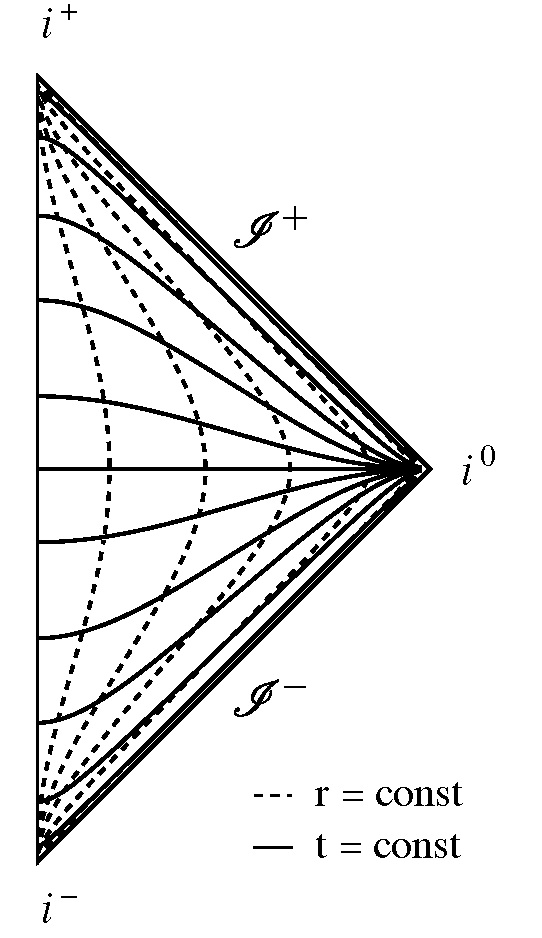
\includegraphics[width =0.3\textwidth]{Penrose diagram.pdf}
    \caption{Penrose Diagram - Representation of the standard
      compactification of the Minkowski spacetime alongside the curves of constant
      time, solid black lines, and the curves of constant r, dotted
      black lines.}
\end{figure}
\\
Additionally, H. Friedrich proposed another conformal representation of Minkowski spacetime specifically adapted for spatial infinity, which will be one used in this work. By applying the following change of coordinates $\tilde{t} = \frac{\tau}{\rho(1-\tau^{2})}$, \enspace $\tilde{\rho} = \frac{1}{\rho(1-\tau^{2})}$ we arrive at this representation. Therefore,
$$ \gamma=-d \tau^2+\frac{\left(1-\tau^2\right)}{\rho^2} d\rho^2-\frac{\tau}{\rho}(d \rho d \tau+d \tau d \rho)+d \Omega^2 $$
We are now in the position to say that the conformal factor $\Theta$ is given by,
\begin{equation}\label{eq:gamma}
	\gamma = \Theta^2 \tilde{\eta}.
\end{equation}
\begin{equation}\label{eq:conf-factor}
	\Theta = \rho(1-\tau^2).
\end{equation}
As a result of the spacetime admitting only particles that travel slower than the speed of light, which in geometric units corresponds to $\pm 1$, hence, we have  
$$ -1 \le \tau \le 1 $$ 
with $\rho$ > 0. Therefore, light travels towards infinity to the places where $\tau = \pm 1$ in the conformal extension. So, in this representation,
$$ \mathscr{I}^+ \equiv \{ \tau = 1 \}, \enspace \mathscr{I}^- \equiv \{ \tau = -1 \}$$ 
The sets where future and past null-infinities touch spatial infinity are named the critical sets and are given by,
$$ \mathcal{I}^+ = \{ \tau = 1, \enspace \rho = 0\}, \enspace \mathcal{I}^- = \{ \tau = -1, \enspace \rho = 0\}$$

%%%%%%%%%%%%%%%%%%%%%%%%%%%%%%%%%%%%%%%%%%%%%%%%%%%%%%%%%%%%%%%%%%%%%%%%
\section{Newman-Penrose Constants}
\label{section:objectives}
The Newman-Penrose constants, originally introduced in \cite{NewPen68}, are quantities defined on null-infinity that obey conservation laws for asymptotically flat gravitational fields. In flat spacetime, there exists an infinite number of conservation laws for each spin value. For example, in ordinary Electromagnetic (EM) theory with a spin-1 field, the total charge is conserved. In the linearized gravitational theory, which involves a spin-2 field, the total mass, linear momentum, and angular momentum are also conserved. In our case, we are interested in studying spin-0 fields, which correspond to solutions of the wave equation.
\\
The NP constants form an infinite hierarchy of conserved quantities for linear equations, including the spin-1, spin-2, and spin-0 fields. Newman and Penrose demonstrated that these constants can be expressed as the product of the square of the dipole moment and the difference between the monopole and the quadrupole moments, as shown in \cite{DaiVal02}. However, in the full non-linear gravitational theory, the conservation of mass and momentum no longer holds, leading to ten distinct conserved quantities.
\\
One intriguing question is whether the NP constants are zero for stationary spacetimes. Remarkably, for the Kerr solution and the Schwarzschild spacetime, the NP constants do vanish \cite{Bac10}, \cite{BaiZhoGonXueXiaoLau07}. The magnitude of these constants provides insights into the residual radiation present in the spacetime following a black hole collision \cite{DaiVal02}. As the NP constants retain their values along null-infinity, they offer valuable information about the behavior of black hole collisions at later times.
\\
Turning our attention to the interpretation of these charges, the NP constants are considered a set of conserved charges at null infinity \cite{NewPen68}. These charges are computed as 2-surface integrals at cuts $\mathcal{C} \approx \mathbb{S}^2$ of null infinity $\mathscr{I}$. In the linear theory, an infinite hierarchy of these conserved quantities exists, while in the non-linear theory of General Relativity, only ten quantities remain conserved \cite{NewPen68}.
\\
The interpretation of these charges is still a subject of debate [\cite{PenRin84}, \cite{DaiVal02}, \cite{Bac10}]. However, their conservation holds in general asymptotically flat spacetimes, even when the dynamics involve complex phenomena like black hole collisions \cite{DaiVal02}. Recent interest in asymptotic quantities, particularly the Bondi-Metzner-Sachs (BMS) charges, has emerged due to their connection with the concept of black hole soft hair [\cite{HawMalStr16}, \cite{HawMalStr17}, \cite{HeLyMi15}]. Understanding the relationship between conserved quantities at past and future null infinity is a crucial aspect of these discussions. However, the resolution of the singular nature of spatial infinity poses challenges in matching the conserved quantities.
\\
Therefore, the study of the Newman-Penrose constants and their conservation offers valuable insights into the dynamics of gravitational fields, particularly in black hole collisions and asymptotically flat spacetimes. These constants provide information about the residual radiation and behavior of the system at later times, shedding light on the intricate nature of spacetime and the conservation laws that govern it.
\\
The Peeling theorem, one of the most emblematic results in the classical theory of asymptotics in general relativity, has played a very important role in the development of the modern notion of gravitational radiation. It is usually formulated within the context of asymptotically simple spacetimes, as defined in Section 10.2 of \cite{Val16}.
\\
An inspection of the proof of the Peeling Theorem reveals that, in fact, it is only necessary to assume that the conformal extension is $C^{4}$.  In view of this, the question of the existence and genericity of spacetimes satisfying the peeling behavior can be rephrased in terms of the construction of asymptotically flat spacetimes with, at least, this minimum of differentiability \cite{GasVal17}. Penrose's compactification procedure, when applied to the Minkowski spacetime, yields a fully smooth conformal extension. However, for spacetimes with nonvanishing mass, such as the Schwarzschild spacetime, the conformal structure degenerates at spatial infinity. This degeneration occurs because spatial infinity can be viewed as the final point of the generators of null infinity, either in the past or future direction. As a result, it is natural to expect that the behavior of the gravitational fields near spatial infinity will somehow reflect the peeling properties of the spacetime \cite{Pen65a}.
\\
The peeling Theorem, documented in [\cite{Sac61}, \cite{BonBurMet62}, \cite{NewPen62}], represents a significant outcome in the study of asymptotic behavior in general relativity. It characterizes the decay of the Weyl tensor in the asymptotic region of the spacetime, signifying the gradual "peeling" of gravitational radiation. This theorem deepens our understanding of the intricate nature of gravitational radiation and its properties in the far-reaching regions of the spacetime.
\\
Hence, the Peeling Theorem, by decomposing the Weyl tensor into NP scalars, and the Newman-Penrose constants, by quantifying and conserving the asymptotic charges at null infinity, are interconnected concepts that deepen our understanding of the gravitational radiation and its properties in asymptotically flat spacetimes.
%%%%%%%%%%%%%%%%%%%%%%%%%%%%%%%%%%%%%%%%%%%%%%%%%%%%%%%%%%%%%%%%%%%%%%%%

\cleardoublepage

%\input{Thesis_new_file} % add new .tex files for new chapters
%\cleardoublepage


% ----------------------------------------------------------------------
%  Bibliography
% ----------------------------------------------------------------------

% Add entry in the table of contents as chapter
\phantomsection
\addcontentsline{toc}{chapter}{\bibname}

% Include all references in .bib file, even non-cited ones...
\nocite{*} % this should be used carefully because it is not correct!

% Produces the bibliography section when processed by BibTeX
%
% Bibliography style
% > entries ordered alphabetically
%\bibliographystyle{plain}
% > unsorted with entries appearing in the order in which the citations appear.
%\bibliographystyle{unsrt}
% > entries ordered alphabetically, with first names and names of journals and months abbreviated
%\bibliographystyle{abbrv}
% > entries ordered alphabetically, with reference markers based on authors' initials and publication year
%\bibliographystyle{alpha}
%
% Replacement bibliography styles provided by 'natbib' package
% (plainnat.bst, abbrvnat.bst, unsrtnat.bst )
% > entries ordered alphabetically
%\bibliographystyle{plainnat}
% > unsorted with entries appearing in the order in which the citations appear.
%\bibliographystyle{unsrtnat}
% > entries ordered alphabetically, with first names and names of journals and months abbreviated
%\bibliographystyle{abbrvnat} % <<<<< SELECT IF USING REFERENCES BY AUTHOR/YEAR
% > entries ordered alphabetically, with reference markers based on authors' initials and publication year
%\bibliographystyle{alpha}
%
% Custom bibliography style adapted from 'natbib' package
%   (based on http://tex.stackexchange.com/questions/5053/is-it-possible-to-get-unsrt-abbrv-bibliography)
%   (unsrtnat.bst + abbrvnat.bst -> abbrvunsrtnat.bst)
%   (original files copied from:
%   http://tug.ctan.org/macros/latex/contrib/natbib/abbrvnat.bst
%   http://tug.ctan.org/macros/latex/contrib/natbib/unsrtnat.bst
% > unsorted with entries appearing in the order in which the citations appear, with first names and names of journals and months abbreviated.
\bibliographystyle{abbrvunsrtnat} % <<<<< SELECT IF USING REFERENCES BY NUMBER (CITATION ORDER)

% External bibliography database file in the BibTeX format
\bibliography{Thesis} % file "Thesis_bib_DB.bib"

\cleardoublepage

% ----------------------------------------------------------------------
%  Appendix (optional)
%
%  CAUTION: 1) the main document (up to the conclusions) shall not exceed 80 pages
%           2) the document shall not exceed a total of 100 pages (per IST regulations)
% ----------------------------------------------------------------------
\appendix

% add page number prefix according to apendix chapter (optional)
%\renewcommand{\thepage}{\thechapter.\arabic{page}}

% re-set arabic numbering (A.1,A.2,...) (optional, use only if chapter prefix is added)
%\setcounter{page}{1}

%%%%%%%%%%%%%%%%%%%%%%%%%%%%%%%%%%%%%%%%%%%%%%%%%%%%%%%%%%%%%%%%%%%%%%%%
%                                                                      %
%     File: Thesis_Appendix_A.tex                                      %
%     Tex Master: Thesis.tex                                           %
%                                                                      %
%     Author: Andre C. Marta                                           %
%     Last modified :  2 Jul 2015                                      %
%                                                                      %
%%%%%%%%%%%%%%%%%%%%%%%%%%%%%%%%%%%%%%%%%%%%%%%%%%%%%%%%%%%%%%%%%%%%%%%%

\chapter{Vector calculus}
\label{chapter:appendixVectors}

In case an appendix if deemed necessary, the document cannot exceed a total of 100 pages...

Some definitions and vector identities are listed in the section below.

% ----------------------------------------------------------------------
\section{Vector identities}
\label{section:vectorIdentities}

\begin{equation}
	\nabla \times \left( \nabla \phi \right) = 0
	\label{eq:cross_nnp}
\end{equation}

\begin{equation}
	\nabla \cdot \left( \nabla \times {\bf u} \right) = 0
	\label{eq:dotCross_nnu}
\end{equation}

 % file "Thesis_Appendix_A.tex"
\cleardoublepage

% re-set arabic numbering (B.1,B.2,...) (optional, use only if chapter prefix is added)
%\setcounter{page}{1}

%%%%%%%%%%%%%%%%%%%%%%%%%%%%%%%%%%%%%%%%%%%%%%%%%%%%%%%%%%%%%%%%%%%%%%%%
%                                                                      %
%     File: Thesis_Appendix_B.tex                                      %
%     Tex Master: Thesis.tex                                           %
%                                                                      %
%     Author: Andre C. Marta                                           %
%     Last modified :  2 Jul 2015                                      %
%                                                                      %
%%%%%%%%%%%%%%%%%%%%%%%%%%%%%%%%%%%%%%%%%%%%%%%%%%%%%%%%%%%%%%%%%%%%%%%%

\chapter{Technical Datasheets}
\label{chapter:appendixDatasheets}

It is possible to add PDF files to the document, such as technical sheets of some equipment used in the work.

% ----------------------------------------------------------------------
\section{Some Datasheet}
\label{section:datasheet}

% See more options to include PDF files in
% http://mirror.unl.edu/ctan/macros/latex/contrib/pdfpages/pdfpages.pdf


 % file "Thesis_Appendix_B.tex"
\cleardoublepage

% ----------------------------------------------------------------------
\end{document}
% ----------------------------------------------------------------------

